% ******** Приклад оформлення документа за ДСТУ 3008-95 ********
% ******************** автор: Тавров Д. Ю. *********************

% зазначаємо стильовий файл, який будемо використовувати
\documentclass{udstu}

% починаємо верстку документа
\begin{document}

% створимо титульний аркуш
% за допомогою спеціальної команди
% \maketitlepage{params},
% де params --- це розділені комами пари "параметр={значення}"
\maketitlepage{
% StudentName --- прізвище, ініціали студента
	StudentName={Скорденко Д. О.},
% StudentMale --- стать студента (true, якщо чоловік, false --- якщо жінка)
	StudentMale=true,
% StudentGroup --- група студента
	StudentGroup={КМ-01},
% Title --- назва
	Title={Звіт\\із лабораторної роботи №4\\із дисципліни \invcommas{Розподілені і хмарні обчислення}},
% SupervisorDegree --- науковий ступінь, учене звання керівника роботи
% якщо наукового ступеня немає, можна відповідний рядочок пропустити
	SupervisorDegree={доцент кафедри ПМА},
% SupervisorName --- прізвище, ініціали керівника роботи
	SupervisorName={Ліскін В. О.}
}

% створюємо зміст
\tableofcontents

% створюємо вступ
\intro

\paragraph{\textbf{Мета:}} розпаралелити метод Гаусса для вирішення СЛАР.

Дослідний приклад:
\begin{equation*}
	A = \begin{bmatrix}
			8 & 7 & 3 \\
			-7 & -4 & -4 \\
			-6 & -5 & -4 \\
	    \end{bmatrix}
	\\
	b = \begin{bmatrix}
			18 \\
			-11 \\
			-15 \\
	    \end{bmatrix}
\end{equation*}

Рішення:
\begin{equation*}
X = \begin{bmatrix}
		5 \\
		-1 \\
		-5 \\
	\end{bmatrix}
\end{equation*}



% створюємо перший розділ роботи
\chapter{Основна частина}
\label{chap:1}

\paragraph{\textbf{Опис програми:}}

Для реалізації паралелізму буде використовуватись 'Rayon'.
Для порівняння швидоксті обчислень буде використовуватись 'Criterion'.
Для матриць / векторів буде використовуватись 'ndarray'.

Порівняння буде проведено на різних к-стях відрізків $n \in [10, 100, 1000]$,
та при різній к-сті потоків $nworkers \in [1,2,4,8]$


\chapter{Опис програми [Тестовий приклад]}
\label{chap:3}

\begin{figure}[!htp]
	\centering
	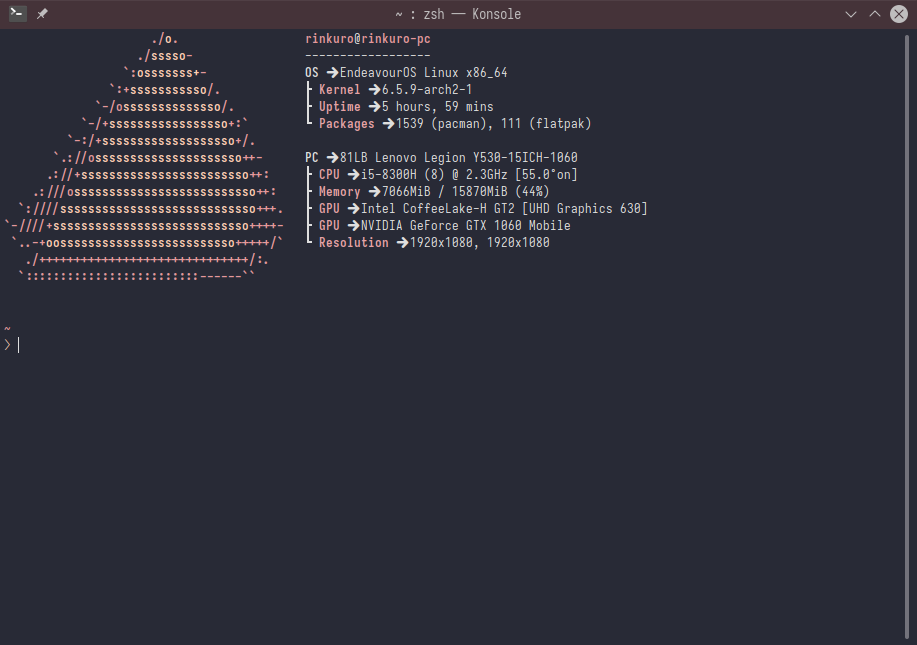
\includegraphics[scale=0.5]{PNG/system-specs.png}
	\caption{Характеристики системи}
	\label{fig:figure1}
\end{figure}

\begin{figure}[!htp]
	\centering
	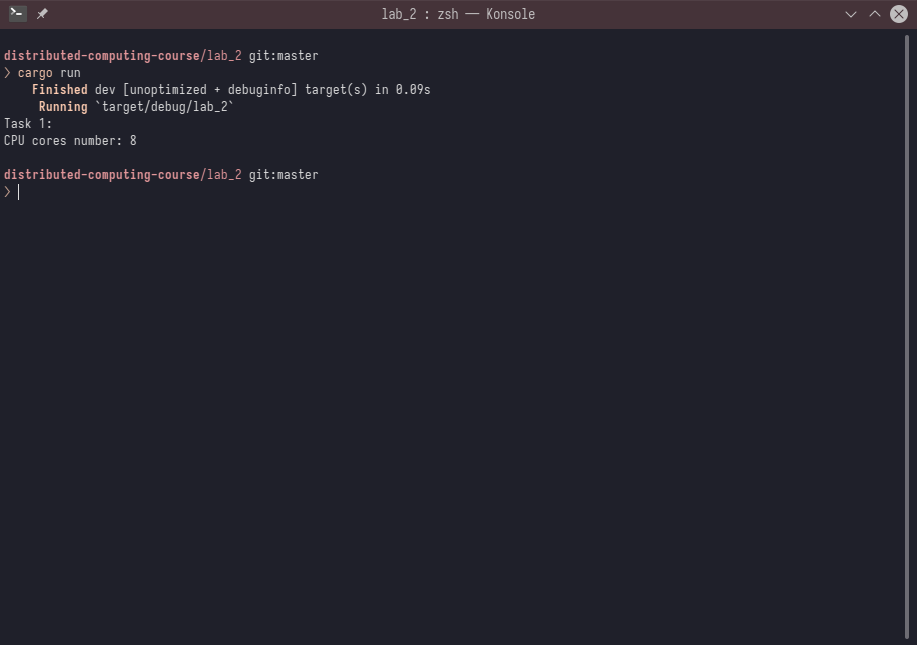
\includegraphics[scale=0.5]{PNG/thread-num-test.png}
	\caption{К-сть ядер процесора}
	\label{fig:figure1}
\end{figure}

\begin{center}
\captionof{table}{Порівняння швидкодії}
\resizebox{\textwidth}{!}{
\begin{tabular}{ | c | c | c | }
	\hline
	n & nworkers & time \\
	\hline
	10 & 1 & 10.621 µs	10.930 µs	11.370 µs \\
	10 & 2 & 17.354 µs	17.776 µs	18.270 µs \\
	10 & 4 & 32.124 µs	32.884 µs	33.736 µs \\
	10 & 8 & 54.917 µs	55.216 µs	55.558 µs \\
	100 & 1 & 1.5261 ms	1.5530 ms	1.5841 ms \\
	100 & 2 & 1.6093 ms	1.6221 ms	1.6357 ms \\
	100 & 4 & 1.9064 ms	1.9908 ms	2.0801 ms \\
	100 & 8 & 2.6843 ms	2.7242 ms	2.7629 ms \\
	1000 & 1 & 1.7285 s	1.7489 s	1.7719 s \\
	1000 & 2 & 1.2366 s	1.2536 s	1.2761 s \\
	1000 & 4 & 1.0471 s	1.0660 s	1.0836 s \\
	1000 & 8 & 987.86 ms	994.92 ms	1.0031 s \\
	\hline
\end{tabular}
}
\end{center}

% створюємо Висновки
\conclusions

На малих об'ємах обчислень збільшення к-сті потоків призводить до погіршення продуктивності.

На більших об'ємах збільшення потоків призводить до збільшення продуктивності,
однак після певної к-сті потоків ефект покращення продуктивності стає незначним.

\append{Код лістінги}

\paragraph{\textsc{*Примітка:}}
У код лістингах при копіюванні втрачається форматування (не копіюються пробіли).
Файли прикріплено до цього pdf (вкладка "прикріплені файли").

\captionof{listing}{lineareq.rs}
\embedfile[filespec=lineareq.rs]{../src/lineareq.rs}
\inputminted{rust}{../src/lineareq.rs}

\captionof{listing}{lib.rs}
\embedfile[filespec=lib.rs]{../src/lib.rs}
\inputminted{rust}{../src/lib.rs}

\captionof{listing}{main.rs}
\embedfile[filespec=main.rs]{../src/main.rs}
\inputminted{rust}{../src/main.rs}

\end{document}
